This chapter builds on the previous to investigate the performance effects of different caching architectures and recovery mechanisms for NVRAM.
I introduce a methodology for evaluating database performance with upcoming NVRAMs and look at NVRAM read and write performance concerns separately.

\section{Methodology}
\label{sec:OLTP_design:Methodology}

This section details the methodology for benchmarking transaction processing and modeling NVRAM performance.
Experiments use the Shore-MT storage manager \cite{JohnsonPandis09}, including the high performance, scalable WAL implementation provided by Aether \cite{JohnsonPandis10}.
While Aether provides a distributed log suitable for multi-socket servers, the distributed log exists as a fork of the main Shore-MT project.
Instead, I limit experiments to a single CPU socket to provide a fair comparison between WAL and other recovery schemes, enforced using the Linux \emph{taskset} utility.
Experiments place both the Shore-MT log and volume files on an in-memory \emph{tmpfs}, and provide sufficiently large buffer caches such that all pages hit in the cache after warmup.
The intent is to allow the database to perform data accesses at DRAM speed and introduce additional delays to model NVRAM performance.
Table~\ref{table::Specs} shows the experimental system configuration.

\begin{table}
  \centering
  \begin{tabular}{l l}
    \hline
    Operating System & Ubuntu 12.04 \\
    CPU & Intel Xeon E5645 \\
    & 2.40 GHz \\
    CPU cores & 6 (12 with HyperThreading) \\
    Memory & 32 GB \\
    \hline
  \end{tabular}
  \caption{\textbf{Experimental system configuration.}}
  \label{table::Specs}
\end{table}

\textbf{Modeling NVRAM delays.}
Since NVRAM devices are not yet available, I must provide a timing model that mimics their expected performance characteristics.
I model NVRAM read and write delays by instrumenting Shore-MT with precisely controlled assembly-code delay loops to model additional NVRAM latency and bandwidth constraints at 13ns precision.
Hence, Shore-MT runs in real time as if its buffer cache resided in NVRAM with the desired read and write characteristics.

I introduce NVRAM delays using the x86 RDTSCP instruction, which returns a CPU-frequency-invariant, monotonically increasing time-stamp that increments each clock tick.
RDTSCP is a synchronous instruction---it does not allow other instructions to reorder with it.
The RDTSCP loop delays threads in increments of 13ns (latency per loop iteration and RDTSCP) with an accuracy of 2ns.

\begin{figure}
  \centering
  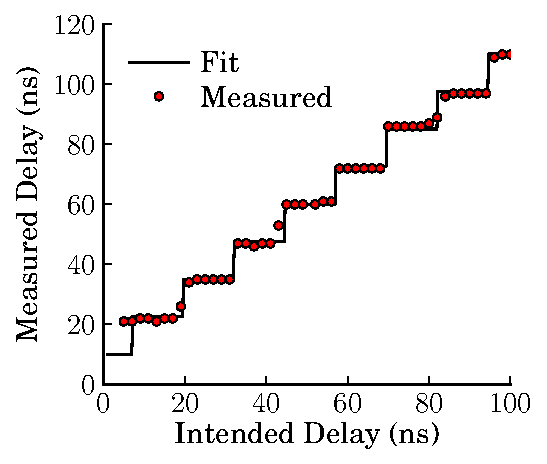
\includegraphics[width=.50\linewidth]{OLTP_eval/Delay.pdf}
  \caption{\textbf{Delay precision.} Delays are implemented by repeatedly reading the TSC register.  Resulting delays form a step function.  Inserted delays are within 6ns of the intended delay.}
  \label{fig::Delay}
\end{figure}

Figure~\ref{fig::Delay} shows the measured delay that results from iterating on an intended delay (both in ns).
Points show the median of ten thousand delay trials (a small number of trials result in excessively large delays, likely due to context switches, and skew the mean).
The delay function resembles a step function---delays may only be inserted in multiples of the loop iteration latency.

To better understand delay behavior I perform a least squares regression of a step function against the measured data of the form:
$$delay(intended) = a \times floor(intended / a + b) + c$$
which results in an $R^2$ of .997 and the following parameter values: $a = 12.5$, $b=.434$, and $c=10.1$.
This indicates that each iteration takes 12.5ns.

As delays can only be introduced in steps I subtract 9.3ns from the intended delay to match the intended delay to the closest step.
The resulting delay is within 6.25ns of the intended delay.
However, a given delay contains a constant skew (for example, an intended delay of 30ns always results in a 35ns delay).
As NVRAM persist latencies are expected to be in the hundreds of ns or greater, such error will negligibly affect my results.

\textbf{Modeling NVRAM persist bandwidth.}
In addition to NVRAM latency, I model shared NVRAM write bandwidth.
Using RDTSCP as a clock source, I maintain a shared \emph{next\_available} variable, representing the next clock tick in which the NVRAM device is available to be written.
Each NVRAM persist advances \emph{next\_available} to account for the latency of its persist operation.
Reservations take the maximum of \emph{next\_available} and the current RDTSCP and add the reservation duration.
The new value is atomically swapped into \emph{next\_available} via a Compare-And-Swap (CAS).
If the CAS fails (due to a race with a persist operation on another thread), the process repeats until it succeeds.
Upon success, the thread delays until the end of its reservation.
The main limitation of this approach is that it cannot model reservations shorter than the delay required to perform a CAS to a contended shared variable.
This technique models reservations above 120ns accurately, which is sufficient for my experiments.

Several factors affect the speed of bandwidth reservations (and therefore reservation accuracy) including the number of threads and their placement across sockets and cores.
I test the reservation system's accuracy by constraining thread placement while threads repeatedly reserve time and delay until the end of the reservation.
It all available time is reserved, reservation overhead is negligible and the modeled bandwidth is accurate.
However, when reservation length is sufficiently short reservation overheads will dominate, resulting in unreserved time.

\begin{table*}
  \centering
  \subtable[6 threads]{
    \label{table::Reservation::6}
    \begin{tabular}{l l l}
      \hline
      socket policy & spread cores & pack cores \\
      \hline \hline
      spread & 109 & 122 \\
      pack & 44 & 104 \\
      \hline
      \\
    \end{tabular}
  }
  \subtable[12 threads]{
    \label{table::Reservation::12}
    \begin{tabular}{l l l}
      \hline
      socket policy & spread cores & pack cores \\
      \hline \hline
      spread & 96 & 101 \\
      pack & 51 & 51 \\
      \hline
      \\
    \end{tabular}
  }
  \caption{\textbf{Bandwidth reservation bendmark.} Benchmark repeatedly reserves bandwidth as time and delays until end of the reservation.  Reservations are inaccurate if entire time cannot be reserved (reservation overhead dominates).  Results shown are reservation sizes (in ns) to reserve 99\% time.  We vary thread placement across CPU sockets and cores: packed (fill socket/core before allocating new) or spread (round robin assign to resources).  122ns and greater reservations accurately model constrained bandwidth.}
  \label{table::Reservation}
\end{table*}


Table~\ref{table::Reservation} shows the required reservation length (in ns) to reserve 99\% of time with six and 12 threads.
Additionally, the Table shows different thread placement across sockets and cores.
``Spread" implies assigning threads round-robin to all available resources, while ``pack" indicates that each resource is filled before assigning any threads to the next.
For example, assigning six threads in a pack sockets--spread cores policy (on a two socket server, each with six cores and two-way SMT) results in all six threads scheduled on the same socket but each thread on its own core (thus SMT is unused).
Such a configuration requires reservations of only 44ns to reserve 99\% of bandwidth-time.

Spreading threads across sockets or packing within cores slows reservations by requiring long-latency communication between sockets or forcing threads to contend with each other while scheduling instructions on cores.
At worst, when threads are spread across sockets and packed within cores a reservation length of 122ns is required to reserve 99\% of time.

A similar trend is true when considering 12 threads.
Packing threads into a socket completely fills all cores and SMT contexts of the socket (the bottom two cells represent the same configuration), needing 51ns reservations for accurate bandwidth modeling.
Spreading threads across sockets while packing cores requires 101ns to reserve 99\% of time.
The required time decreases from six to 12 threads as more threads are available to reserve time and it is less likely that time will go unreserved.

These results suggest that bandwidth reservations will be accurate so long as each reservation exceeds 120ns.
In Shore-MT I reserve bandwidth for each cache line persisted.
The persist bandwidth analysis study (presented later in Section~\ref{sec:OLTP_eval:Persists:Limitations}) shows that 35ns per cache line (approximately 1.7GB/s persists) represents sufficient bandwidth to negligibly limit performance.
Since at least four cache lines are always reserved together (in \texttt{persist\_page} and \texttt{persist\_wal}) the bandwidth reservation is accurate.

\textbf{NVRAM performance.}
I introduce NVRAM read and write delays separately.
Accurately modeling per-access increases in read latency is challenging, as reads are frequent and the expected latency increases on NVRAM are small.
It is infeasible to use software instrumentation to model such latency increases at the granularity of individual reads; hardware support, substantial time dilation, or alternative evaluation techniques (e.g., simulation) would be required, all of which compromise accuracy and the ability to run experiments at full scale.
Instead, I use offline analysis with PIN \cite{LukCohn05} to determine (1) the reuse statistics of buffer cache pages, and (2) the average number of cache lines accessed each time a page is latched.
Together, these offline statistics provide an average number of cache line accesses per page latch event in Shore-MT while considering the effects of page caching.
I then introduce a delay at each latch based on the measured average number of misses and an assumed per-read latency increase based on the NVRAM technology.

I model NVRAM persist delays by annotating Shore-MT to track buffer cache writes at cache line granularity---64 bytes---using efficient ``dirty" bitmaps.
Depending on the recovery mechanism, I introduce delays corresponding to persist barriers and to model NVRAM write bandwidth contention.
Tracking buffer cache writes introduces less than a 3\% overhead to the highest throughput experiments.

I choose on-line timing modeling via software instrumentation in lieu of architectural simulations to allow experiments to execute at full scale and in real time.
While modeling aspects of NVRAM systems such as cache performance and more precise persist barrier delays require detailed hardware simulation, I believe NVRAM device and memory system design are not sufficiently established to consider this level of detail.
Instead, I investigate more general trends to determine if and when NVRAM read and write performance warrant storage management redesign.

\textbf{Recovery performance.} Figure~\ref{fig::Recovery} displays recovery latency vs transaction throughput for the TPCB workload, varying page flush rate.
Page flush rate is controlled by maintaining a constant number of dirty pages in the buffer cache, always flushing the page with the oldest volatile update.
Experiments run TPCB for one minute (sufficient to reach steady state behavior) and then kill the Shore-MT process.
Before starting recovery I drop the file system cache.
Reported recovery time includes only the recovery portion of the Shore-MT process; I do not include system startup time nor non-recovery Shore-MT startup time.

\textbf{Workloads}
I use three workloads and transactions in this evaluation: TPCC, TPCB, and TATP.
TPCC models order management for a company providing a product or service \cite{TPCC}.
TPCB contains one transaction class and models a bank executing transactions across branches, tellers, customers, and accounts \cite{TPCB}.
TATP includes seven transactions to model a Home Location Registry used by mobile carriers \cite{TATP}.
Table~\ref{table::Workloads} shows the workload configuration.
%I choose a single updating transaction from each workload and size workloads to fit in a 12GB buffer cache.
I scale workloads to fit in a 12GB buffer cache.
Persist performance experiments use a single write-heavy transaction from each workload while read performance experiments use each workload's full mix.
All experiments report throughput as thousands of Transactions Per Second (kTPS).
Experiments perform ``power runs" -- each thread generates and executes transactions continuously without think time -- and run an optimal number of threads per configuration (between 10 and 12).

\begin{table}
  \centering
  \begin{tabular}{l l l l}
    \hline
    Workload & Scale factor & Size & Write transaction \\
    \hline \hline
    TPCC & 70 & 9GB & New order \\
    TPCB & 1000 & 11GB & \\
    TATP & 600 & 10GB & Update location \\
    \hline
  \end{tabular}
  \caption{\textbf{Workloads and transactions.}  One transaction class from each of three workloads, sized to approximately 10GB.}
  \label{table::Workloads}
\end{table}

\section{NVRAM Reads}
\label{sec:OLTP_eval:Reads}

I first evaluate database performance with respect to NVRAM reads.
Many candidate NVRAM technologies exhibit greater read latency than DRAM, possibly requiring additional hardware or software caching.
I wish to determine, for a given NVRAM read latency, how much caching is necessary to prevent slowdown, and whether it is feasible to provide this capacity in a hardware-controlled cache (otherwise software caches must be used).

\subsection{NVRAM Caching Performance}
\label{sec:OLTP_eval:Reads:Performance}

\textbf{Traces.}
\begin{table*}
  \centering
  \begin{tabulary}{\textwidth}{L L L L L L L L L}
    \hline
    & \multicolumn{2}{c}{TATP} & \multicolumn{2}{c}{TPCB} & \multicolumn{2}{c}{TPCC} & \multicolumn{2}{c}{Average} \\
    & \% lines & lines/latch & \% lines & lines/latch & \% lines & lines/latch & \% lines & lines/latch \\
    \hline \hline
    Store & 10.57\% & 5.32 & 11.71\% & 6.05 & 15.47\% &  4.25 & 12.58\% & 5.20 \\
    Index & 89.43\% & 11.27 & 82.41\% & 12.19 & 81.18\% & 11.17 & 84.34\% & 11.54 \\
    Other & 0.00\% & 0.00 & 5.89\% & 7.16 & 3.36\% & 3.00 & 3.08\% & 3.39 \\
    Total & & 5.53 & & 8.47 & & 6.14 & & 6.71 \\
    \hline
  \end{tabulary}
  \caption{\textbf{NVRAM access characteristics.} ``\% lines" indicates the percentage breakdown of cache line accesses.  ``lines/latch" reports the average number of cache line accesses per page latch.  Indices represent the majority of accesses.}
  \label{table::AccessCharacteristics}
\end{table*}

The NVRAM read-performance model combines memory access trace analysis with the timing model to measure transaction throughput directly in Shore-MT.
Traces consist of memory accesses to the buffer cache, collected running Shore-MT with PIN for a single transaction thread for two minutes.
I assume concurrent threads exhibit similar access patterns.
In addition, I record all latch events (acquire and release) and latch page information (i.e., table id, store type -- index, heap, or other).
I analyze traces at cache line (64 bytes) and page (8KB) granularity.

These traces provide insight into how Shore-MT accesses persistent data, summarized in Table~\ref{table::AccessCharacteristics}.
Index accesses represent the great majority of cache line accesses, averaging 85\% of accesses to NVRAM across workloads.
Any caching efforts should focus primarily on index pages and cache lines.
Note also that indexes access a greater number of cache lines per page access than other page types (average 11.48 vs 4.85 for heap pages and 4.77 for other page types), suggesting that uncached index page accesses have the potential to introduce greater delays.

\textbf{Throughput.}
\begin{figure}
  \centering
  \subfigure[TATP]{\label{fig::ReadPerformance::TATP} 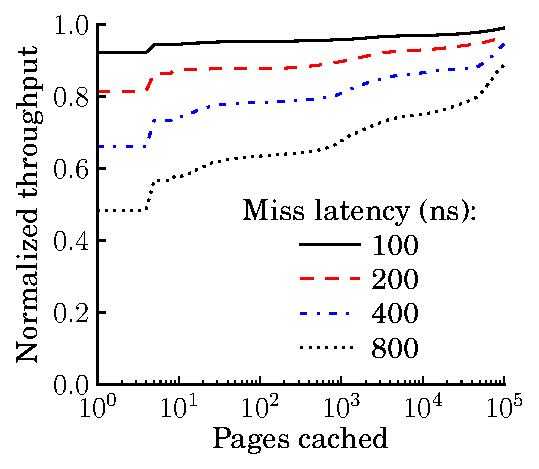
\includegraphics[width=.49\textwidth]{OLTP_eval/ReadPerformance_TATP.pdf}}
  \subfigure[TPCB]{\label{fig::ReadPerformance::TPCB}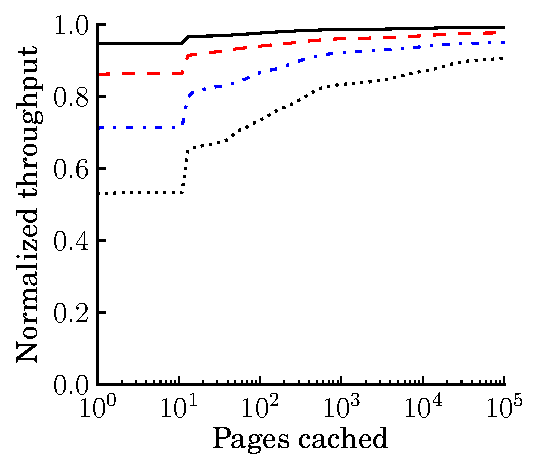
\includegraphics[width=.49\textwidth]{OLTP_eval/ReadPerformance_TPCB.pdf}}
  \subfigure[TPCC]{\label{fig::ReadPerformance::TPCC}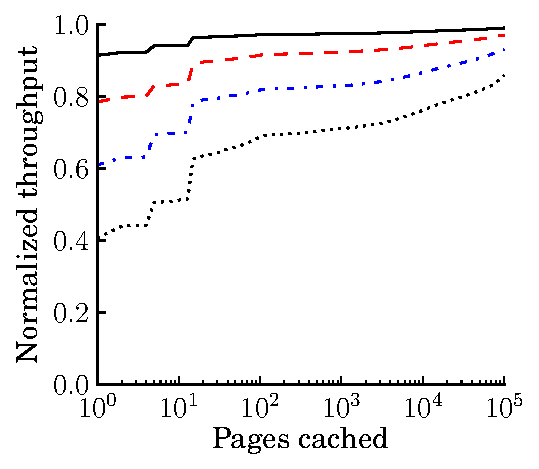
\includegraphics[width=.49\textwidth]{OLTP_eval/ReadPerformance_TPCC.pdf}}
%  \begin{subfigure}{0.32\textwidth}
%    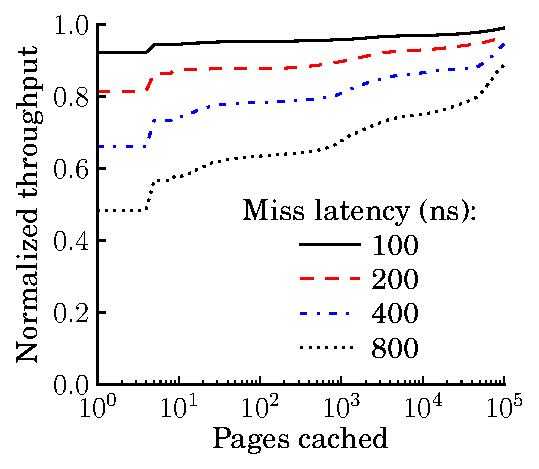
\includegraphics[width=\textwidth]{OLTP_eval/ReadPerformance_TATP.pdf}
%    \caption{TATP}
%    \label{fig::ReadPerformance::TATP}
%  \end{subfigure}
%  \begin{subfigure}{0.32\textwidth}
%    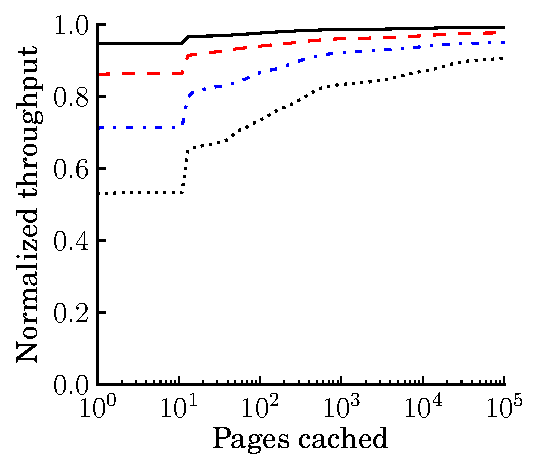
\includegraphics[width=\textwidth]{OLTP_eval/ReadPerformance_TPCB.pdf}
%    \caption{TPCB}
%    \label{fig::ReadPerformance::TPCB}
%  \end{subfigure}
%  \begin{subfigure}{0.32\textwidth}
%    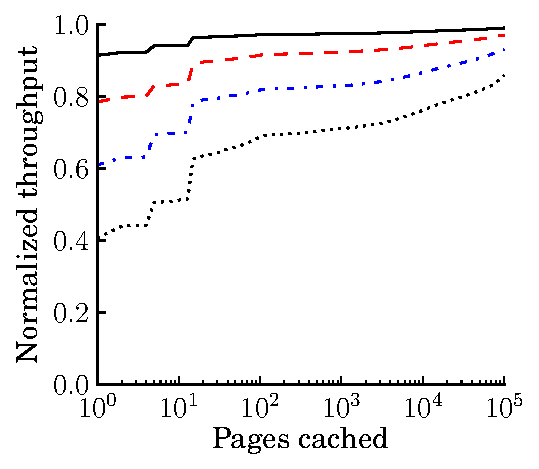
\includegraphics[width=\textwidth]{OLTP_eval/ReadPerformance_TPCC.pdf}
%    \caption{TPCC}
%    \label{fig::ReadPerformance::TPCC}
%  \end{subfigure}
  \caption{\textbf{Throughput vs NVRAM read latency.} 100ns miss latency suffers up to a 10\% slowdown over DRAM.  Higher miss latencies introduce large slowdowns, requiring caching.  Fortunately, even small caches effectively accelerate reads.}
  \label{fig::ReadPerformance}
\end{figure}

I create a timing model in Shore-MT from the previous memory traces.
Given traces, I perform cache analysis at page granularity, treating latches as page accesses and assuming a fully associative cache with a least-recently-used replacement policy (LRU).
Cache analysis produces an average page miss rate to each table.
I conservatively assume that every cache line access within an uncached page introduces an NVRAM stall, neglecting optimizations such as out-of-order execution and simultaneous multi-threading that might hide some NVRAM access stalls. 
The model assumes the test platform incurs a 50ns DRAM fetch latency, and adds additional latency to mimic NVRAM (for example, a 200ns NVRAM access adds 150ns delay per cache line).
I combine average page miss rate and average miss penalty (from lines/latch in table~\ref{table::AccessCharacteristics}) to compute the average delay incurred per latch event.
This delay is inserted at each page latch acquire in Shore-MT, using \InPlace, to produce a corresponding throughput.

Figure~\ref{fig::ReadPerformance} shows throughput achieved for the three workloads while varying the number of pages cached (horizontal axis) and NVRAM miss latency (various lines).
The vertical axis displays throughput normalized to DRAM-miss-latency's throughput (no additional delay inserted).
Without caching, throughput suffers as NVRAM miss latency increases, shown at the extreme left of each graph.
A 100ns miss latency consistently achieves at least 90\% of potential throughput.
However, an 800ns miss latency averages only 50\% of the potential throughput, clearly requiring caching.
TPCB and TPCC see a 10-20\% throughput improvement for a cache size of just 20 pages.
As cache capacity further increases, each workload's throughput improves to varying degrees.
A cache capacity of 100,000 (or 819MB at 8KB pages) allows NVRAMs with 800ns miss latencies to achieve at least 80\% of the potential throughput.
While too large for on-chip caches, such a buffer might be possible as a hardware-managed DRAM cache \cite{QureshiSrinivasan09}.

\subsection{Analysis}
\label{sec:OLTP_eval:Reads:Analysis}
\begin{figure}
  \centering
  \subfigure[TATP]{\label{fig::Caching::TATP} 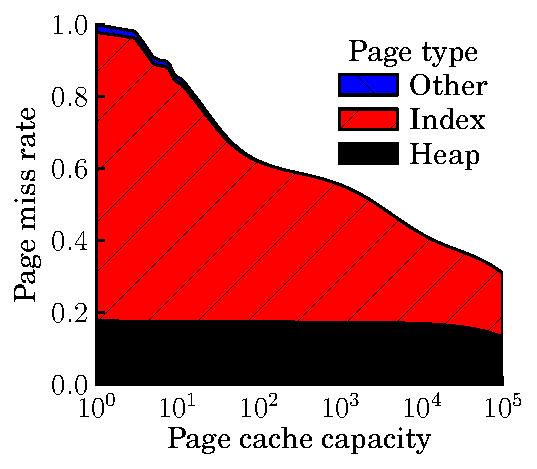
\includegraphics[width=.45\textwidth]{OLTP_eval/Caching_TATP.pdf}}
  \subfigure[TPCB]{\label{fig::Caching::TPCB}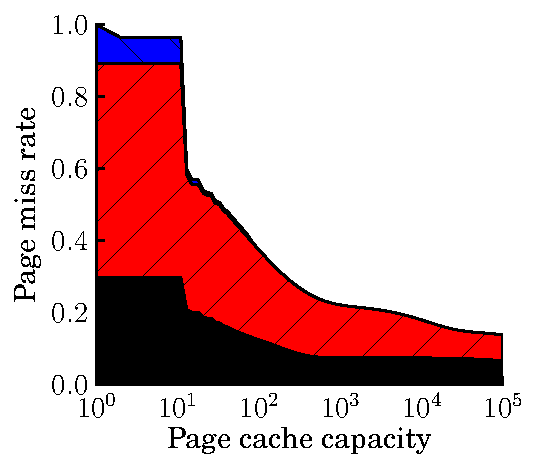
\includegraphics[width=.45\textwidth]{OLTP_eval/Caching_TPCB.pdf}}
  \subfigure[TPCC]{\label{fig::Caching::TPCC}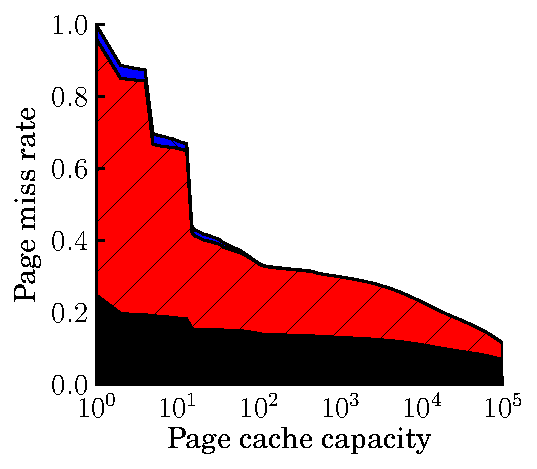
\includegraphics[width=.45\textwidth]{OLTP_eval/Caching_TPCC.pdf}}
  \caption{\textbf{Page caching effectiveness.} High level B+Tree pages and append-heavy store pages cache effectively.  Other pages cache as capacity approaches table size.}
  \label{fig::Caching}
\end{figure}

I have shown that modest cache sizes effectively hide NVRAM read stalls for these workloads, and further analyze caching behavior to reason about OLTP performance more generally.
Figure~\ref{fig::Caching} shows the page miss rate per page type (index, heap, or other) as page cache capacity increases.
Each graph begins at 1.0 at the left---all page accesses miss for a single-page cache.
As cache capacity increases, workloads see their miss rates start to decrease between cache capacity of five and 20 pages.
TATP experiences a decrease in misses primarily in index pages, whereas TPCB and TPCC see a decrease across all page types.

While cache behavior is specific to each workload, the results represent trends applicable to many databases and workloads, specifically, index accesses and append-heavy tables.
First, all workloads see a decrease in index page misses as soon as B+Tree roots (accessed on every traversal) successfully cache.
The hierarchical nature of B+Tree indexes allows high levels of the tree to cache effectively for even a small cache capacity.
Additionally, TPCB and TPCC contain history tables to which data are primarily appended.
Transactions append to the same page as previous transactions, allowing such tables to cache effectively.
Similarly, extent map pages used for allocating new pages and locating pages to append into are frequently accessed and likely to cache.
The remaining tables' pages are accessed randomly and only cache as capacity approaches the size of each table.
In the case of TPCB and TPCC, each transaction touches a random tuple of successively larger tables (Branch, Teller, and Account for TPCB; Warehouse, District, Customer, etc. for TPCC).
This analysis suggests that various page types, notably index and append-heavy pages, cache effectively, accelerating throughput for high-latency NVRAM misses with small cache capacities.

\textbf{Main-memory databases.}
While I use Shore-MT (a disk-based storage manager) as a research platform, main-memory database optimizations (e.g., \cite{DiaconuFreedman13, BallardBehman11, Oracle09}) also apply to byte-addressable NVRAM.
Main-memory databas\-es assume heap data resides solely in byte-addressable memory, improving throughput relative to traditional disk-back\-ed storage by removing expensive indirection (i.e., using memory pointers instead of buffer translation tables), reducing overheads associated with concurrency control and latches, and optimizing data layout for caches and main-memory, among other optimizations.
While such optimizations will increase transaction throughput, removing non-NVRAM overheads will amplify the importance of read-miss latency (an equal increase in NVRAM read-miss latency will yield a relatively greater drop in performance).
At the same time, data layout optimizations will reduce the number of cache lines and memory rows accessed per action (e.g., per latch), minimizing NVRAM read overheads.
Investigating main-memory database optimizations for NVRAM remains future work.

\begin{table}
  \centering
  \begin{tabular}{l l}
    \hline
    Workload & Bandwidth (GB/s) \\
    \hline \hline
    TATP & 0.977 \\
    TPCB & 1.044 \\
    TPCC & 1.168 \\
    \hline
  \end{tabular}
  \caption{\textbf{Required NVRAM read bandwidth.} Workloads require up to 1.2 GB/s read bandwith.}
  \label{table::ReadBandwidth}
\end{table}

\textbf{Bandwidth.}
Finally, I briefly address NVRAM read bandwidth.
For a worst-case analysis, I assume no caching.
Given the average number of cache line accesses per page latch, the average number of page latches per transaction, and transaction throughput (taken from Section~\ref{sec:OLTP_eval:Persists}), I compute worst-case NVRAM read bandwidth for each workload, shown in Table~\ref{table::ReadBandwidth}~
The considered workloads require at most 1.168 GB/s (TPCC).
Since this is lower than expected NVRAM bandwidth and caching reduces the required bandwidth further, I conclude that NVRAM read bandwidth for persistent data on OLTP is not a concern.

\subsection{Summary}
\label{sec:OLTP_eval:Reads:Summary}
NVRAM presents a new storage technology for which modern database systems have not been optimized.
Increased memory read latencies require new consideration for database caching systems.
I show that persistent data for OLTP can be cached effectively, even with limited cache capacity.
I expect future NVRAM software to leverage hardware caches, omitting software buffer caches.
Next, I turn to write performance for storage management on NVRAM devices.

\section{NVRAM Persist Synchronization}
\label{sec:OLTP_eval:Persists}

Whereas NVRAM reads benefit from caching, persists must always access the device.
Of particular insterest is the cost of ordering persists via persist barriers.
Several factors increase persist barrier latency, including ordering persists across distributed/NUMA memory architectures, long latency interconnects (e.g., PCIe-attached storage), and slow NVRAM MLC cell persists.
I consider the effect of persist barrier latency on transaction processing throughput to determine if and when new NVRAM technologies warrant redesigning recovery management.

Refer to Sections~\ref{sec:OLTP_design:Design} and~\ref{sec:OLTP_design:Methodology} for a more thorough description of recovery mechanisms and experimental setup.
All experiments throttle persist bandwidth to 1.5GB/s, which I believe to be conservative (already possible with PCIe-attached Flash).
Ideally, NVRAM will provide low latency access, enabling \InPlace.
However, one would expect \InPlace's performance to suffer at large persist barrier latencies, requiring either \NVDisk or \GroupCommit to regain throughput.

\subsection{Persist Barrier Latency}
\label{sec:OLTP_eval:Persists:Performance}

\begin{figure*}
  \centering
  %\begin{subfigure}{0.32\textwidth}
  %  \includegraphics[width=\textwidth]{figures/pdfs/PersistLatencyThroughput/TATP.pdf}
  %  \caption{TATP}
  %  \label{fig::PersistLatencyThroughput::TATP}
  %\end{subfigure}
  %\begin{subfigure}{0.32\textwidth}
  %  \includegraphics[width=\textwidth]{figures/pdfs/PersistLatencyThroughput/TPCB.pdf}
  %  \caption{TPCB}
  %  \label{fig::PersistLatencyThroughput::TPCB}
  %\end{subfigure}
  %\begin{subfigure}{0.32\textwidth}
  %  \includegraphics[width=\textwidth]{figures/pdfs/PersistLatencyThroughput/TPCC.pdf}
  %  \caption{TPCC}
  %  \label{fig::PersistLatencyThroughput::TPCC}
  %\end{subfigure}
  \subfigure[TATP]{\label{fig::PersistLatencyThroughput::TATP} 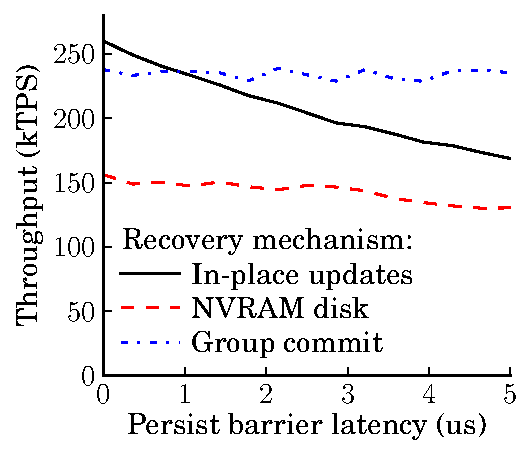
\includegraphics[width=.45\textwidth]{OLTP_eval/PersistLatencyThroughput_TATP.pdf}}
  \subfigure[TPCB]{\label{fig::PersistLatencyThroughput::TPCB}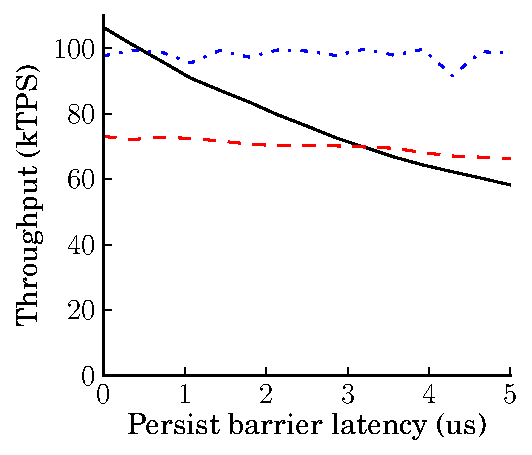
\includegraphics[width=.45\textwidth]{OLTP_eval/PersistLatencyThroughput_TPCB.pdf}}
  \subfigure[TPCC]{\label{fig::PersistLatencyThroughput::TPCC}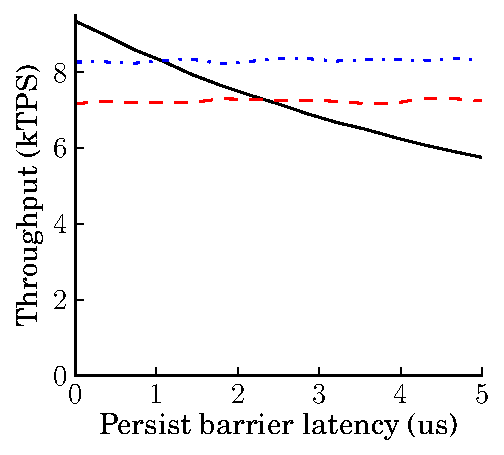
\includegraphics[width=.45\textwidth]{OLTP_eval/PersistLatencyThroughput_TPCC.pdf}}
  \caption{\textbf{Throughput vs persist barrier latency.} \InPlace performs best for zero-cost persist barriers, but throughput suffers as persist barrier latency increases.  \NVDisk and \GroupCommit are both insensitive to increasing persist barrier latency, with \GroupCommit offering higher throughput.}
  \label{fig::PersistLatencyThroughput}
\end{figure*}


Figure~\ref{fig::PersistLatencyThroughput} shows throughput for write-heavy transactions as persist barrier latency increases from 0\textmu s to 5\textmu s, the range believed to encompass realistic latencies for possible implementations of persist barriers and storage architectures.
A persist barrier latency of 0\textmu s (left edge) corresponds to no barrier/DRAM latency.
For such devices (e.g., battery-backed DRAM), \InPlace far out-paces \NVDisk, providing up to a 50\% throughput improvement.
The speedup stems from a combination of removing WAL overheads, removing contention between page flushers and transaction threads, and freeing up (a few) threads from log and page flushers to run additional transactions.
\InPlace also outperforms \GroupCommit, providing an average 10\% throughput improvement across workloads.

As persist barrier latency increases, each recovery mechanism reacts differently.
\InPlace, as expected, loses throughput.
\NVDisk and \GroupCommit, on the other hand, are both insensitive to persist barrier latency; their throughputs see only a small decrease as persist barrier latency increases.
TATP sees the largest throughput decrease for \NVDisk (14\% from 0\textmu s to 5\textmu s).
The decrease stems from \NVDisk's synchronous commits, requiring the log flusher thread to complete flushing before transactions commit.
During this time, transaction threads sit idle.
While both \NVDisk and \GroupCommit retain high throughput, there is a large gap between the two, with \GroupCommit providing up to a 50\% performance improvement over \NVDisk.
This difference, however, is workload dependent, with WAL imposing a greater bottleneck to TATP than to TPCB or TPCC.

Of particular interest are persist barrier latencies where lines intersect---the break-even points for determining the optimal recovery mechanism.
Whereas all workloads prefer \InPlace for a 0\textmu s persist barrier latency, \GroupCommit provides better throughput above 1\textmu s persist barrier latency.
When only considering \InPlace and \NVDisk the decision is less clear.
Over the range of persist barrier latencies TATP always prefers \InPlace to \NVDisk (the break-even latency is well above 5\textmu s).
TPCB and TPCC see the two mechanisms intersect near 3.5\textmu s and 2.5\textmu s, respectively, above which \NVDisk provides higher throughput.
TATP, unlike the other two workloads, only updates a single page per transaction.
Other overheads tend to dominate transaction time, resulting in a relatively shallow \InPlace curve.

\begin{table}
  \centering
  \begin{tabular}{l l l}
    \hline
    Workload & Full mix & Single transaction \\
    \hline \hline
    TATP & 25 & 12 \\
    TPCB & 3.2 & 3.2 \\
    TPCC & 3.6 & 2.4 \\
    \hline
  \end{tabular}
  \caption{\textbf{Break-even persist latency} Persist barrier latency (\textmu s) where \NVDisk and \InPlace achieve equal throughput.  Latencies reported for full transaction mixes and single write-heavy transaction per workload.}
  \label{table::PersistLatencyBreakeven}
\end{table}


The previous results show throughput only for a single transaction from each workload.
Table~\ref{table::PersistLatencyBreakeven} shows break-even persist barrier latency between \NVDisk and \InPlace for these transactions and full transaction mixes.
Full transaction mixes contain read-only transactions, reducing log insert and persist barrier frequency (read-only transactions require no recovery).
\NVDisk sees improved throughput at 0 \textmu s and \InPlace's throughput degrades less quickly as persist barrier latency increases.
As a result, the break-even persist barrier latency between these two designs increases for the full transaction mix relative to a single write-heavy transaction and the opportunity to improve throughput by optimizing recovery management diminishes---improved recovery management does not affect read-only transactions and actions.

These results suggest different conclusions across storage architectures.
NVRAM connected via the main memory bus will provide low latency persist barriers (less than 1\textmu s) and prefer \InPlace.
Other storage architectures, such as distributed storage, require greater delays to synchronize persists.
For such devices, \GroupCommit offers an alternative to \NVDisk that removes software overheads inherent in WAL while providing recovery.
However, \GroupCommit increases transaction latency.

\subsection{Transaction Latency}
\label{sec:OLTP_eval:Persists:XctLatency}

\begin{figure*}
  \centering
  %\begin{subfigure}{0.32\textwidth}
  %  \includegraphics[width=\textwidth]{figures/pdfs/XctLatency/TATP.pdf}
  %  \caption{TATP}
  %  \label{fig::XctLatency::TATP}
  %\end{subfigure}
  %\begin{subfigure}{0.32\textwidth}
  %  \includegraphics[width=\textwidth]{figures/pdfs/XctLatency/TPCB.pdf}
  %  \caption{TPCB}
  %  \label{fig::XctLatency::TPCB}
  %\end{subfigure}
  %\begin{subfigure}{0.32\textwidth}
  %  \includegraphics[width=\textwidth]{figures/pdfs/XctLatency/TPCC.pdf}
  %  \caption{TPCC}
  %  \label{fig::XctLatency::TPCC}
  %\end{subfigure}
  \subfigure[TATP -- Update Location]{\label{fig::XctLatency::TATP} 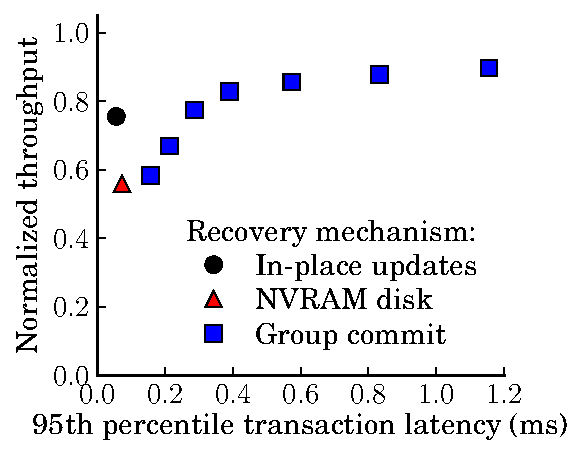
\includegraphics[width=.45\textwidth]{OLTP_eval/XctLatency_TATP.pdf}}
  \subfigure[TPCB]{\label{fig::XctLatency::TPCB}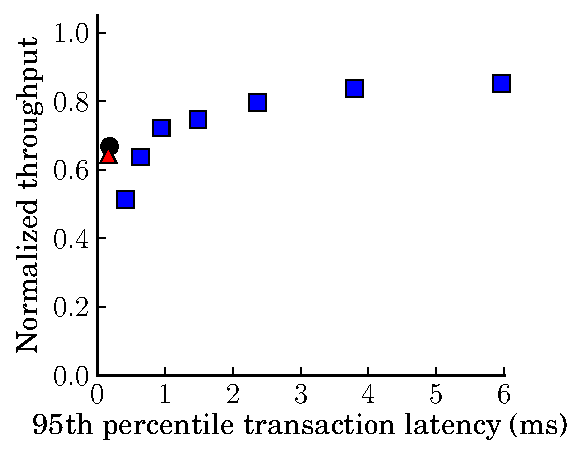
\includegraphics[width=.45\textwidth]{OLTP_eval/XctLatency_TPCB.pdf}}
  \subfigure[TPCC -- New Order]{\label{fig::XctLatency::TPCC}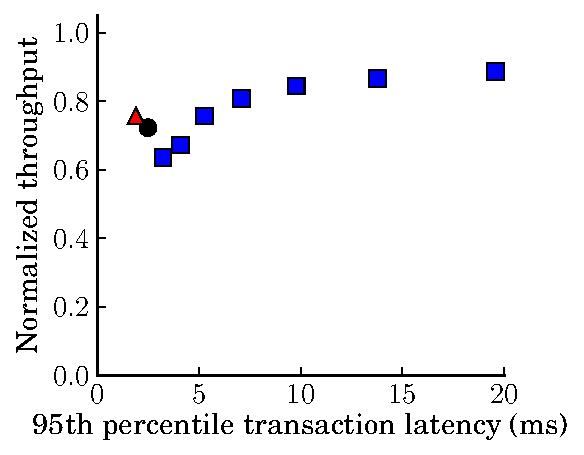
\includegraphics[width=.45\textwidth]{OLTP_eval/XctLatency_TPCC.pdf}}
  \caption{\textbf{95th percentile transaction latency.} All graphs are normalized to 0\textmu s persist barrier latency \InPlace throughput.  Experiments use 3\textmu s persist barrier latency.  \GroupCommit avoids high latency persist barriers by defering transaction commit, committing entire batches atomically.}
  \label{fig::XctLatency}
\end{figure*}


\GroupCommit improves transaction throughput by placing transactions into batches and committing all transactions in a batch atomically.
Doing so minimizes and limits the number of inserted persist barriers.
However, deferring transaction commit increases transaction latency, especially for the earliest transactions in each batch.
To achieve reasonable throughput, batches must be significantly longer than average transaction latency (such that batch execution time dominates batch quiesce and persist time).
The batch period acts as a knob for database administrators to trade off transaction latency and throughput.
I use this knob to measure the relationship between throughput and high-percentile transaction latency.

Figure~\ref{fig::XctLatency} shows throughput, normalized to \InPlace at 0\textmu s persist barrier latency.
The results consider a 3\textmu s persist barrier latency, where \GroupCommit provides a throughput improvement over other recovery mechanisms.
The different \GroupCommit points represent different batch periods, and I report the measured 95th percentile transaction latency for all recovery mechanisms.
I measure transaction latency from the time a transaction begins to the time its batch ends (Shore-MT does not model any pre-transaction queuing time).

The results illustrate that \GroupCommit is capable of providing equivalent throughput to the other recovery mechanisms with reasonable latency increases (no more than 5\texttimes).
Further, high-percentile transaction latencies fall well below the latency expectations of modern applications.
TPCC, the highest latency workload, approaches optimal throughput with a 95th percentile transaction latency of 15ms---similar to latencies incurred by disk-backed databases.
For latency sensitive workloads, the batch period can be selected to precisely control latency, and \InPlace and \NVDisk remain alternatives.

\subsection{NVRAM Persist Limitations}
\label{sec:OLTP_eval:Persists:Limitations}

In addition to persist delays NVRAM may suffer limitations due to persist bandwidth and write endurance.
I quantify these limitations and determine how database design affects each.

\textbf{Persist bandwidth.}
Different NVRAM storage architectures impose a variety of limitations on persist bandwidth (e.g., memory bus-attached NVRAM will allow greater throughput than PCIe-attached NVRAM).
Different software designs place varying requirements on bandwidth.

\begin{figure}
  \centering
  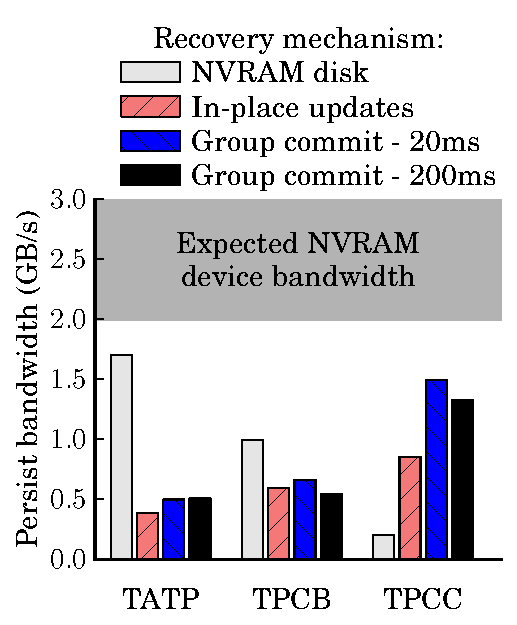
\includegraphics[width=.9\linewidth]{OLTP_eval/Bandwidth.pdf}
  \caption{\textbf{Required NVRAM bandwidth.} Persist/write bandwidth required to achieve 95\% performance relative to no bandwidth constraint.  Bandwidth requirements are far below expected device bandwidth.}
  \label{fig::Bandwidth}
\end{figure}

Figure~\ref{fig::Bandwidth} shows the bandwidth required for each workload and recovery mechanism to achieve 95\% throughput compared to same configuration with no bandwidth constraint.
Each recovery mechanism sees different bandwidth requirements, and required bandwidth varies across workloads.

The \NVDisk configuration flushes pages aggressively (attempts to flush continuously) and consumes all available bandwidth.
Since bandwidth is restricted recovery latency may increase (not reflected in the results).
Page flushing contends with log flushing for bandwidth, but so long as log flushes are minimally delayed throughput will not be affected.
TATP, which contains short transactions, requires the most bandwidth (1.7GB/s) to reduce transaction commit delays.
I believe that asynchronous commit would alleviate this bandwidth requirement.
TPCC, on the other hand, has long transactions and transaction commit is less of a concern.

\InPlace requires the least bandwidth of the recovery mechanisms.
TATP's Update Location transaction needs only 0.4GB/s since each transaction contains a single small update.
TPCC's New Order transaction modifies much more data, requiring 0.8GB/s persist bandwidth to achieve 95\% throughput.

Finally, \GroupCommit sees varying requirements on persist bandwidth.
All persists occur at batch boundaries, resulting in quick persist bursts.
I consider two batch periods---20ms and 200ms.
TATP and TPCC require relatively small bandwidths while TPCC requires over 1.5GB/s persist bandwidth to achieve 95\% throughput.
The bursty nature of \GroupCommit and large modifications by TPCC's New Order transaction result in persist bandwidth quickly creating a bottleneck.
Longer batches help slightly by allowing updates to coalesce within the batch, reducing the total number of bytes persisted.
The bandwidth requirements would be reduced by introducing mechanisms to enable early persists (persist data before the batch ends).

While persist bandwidth requirements vary, the strictest configuration (\NVDisk for TATP) requires only 1.7GB/s.
Such bandwidth is currently possible with existing PCIe Flash memory SSDs, and I believe is attainable for all candidate NVRAM technologies.
Thus, I conclude that persist bandwidth will not be a concern for OLTP systems using NVRAM.

\textbf{Device lifetime.}
NVRAM technologies, much like Flash memory currently, will have limited write endurance; each cell may only be reliably written a finite number of times.
Device lifetime is generally determined by the most frequently written addresses.
Previous work proposes hardware techniques to evenly distribute writes amongst cells by constantly changing the mapping between between memory addresses and the underlying memory cell \cite{QureshiKaridis09}.
These techniques prolong device lifetime by ensuring that frequently written addresses do not wear out individual cells.
While the recovery mechanisms presented here each produce varying persist rates with different abilities to naturally distribute persists across addresses, it is unclear if software mechanisms are sufficient to prolong device lifetime.

\begin{figure*}
  \centering
  \subfigure[No wear leveling]{\label{fig::WearLeveling::None} 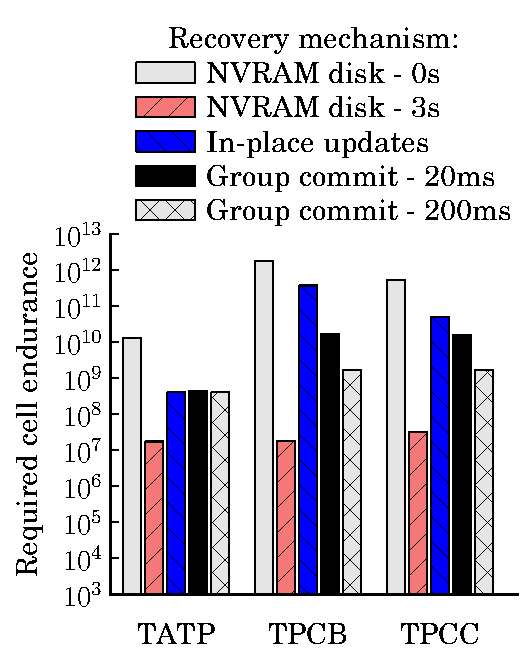
\includegraphics[width=.49\textwidth]{OLTP_eval/WearLeveling_None.pdf}}
  \subfigure[Perfect wear leveling]{\label{fig::WearLeveling::Perfect}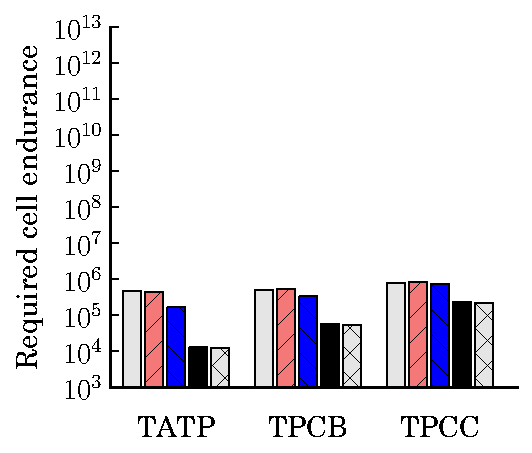
\includegraphics[width=.49\textwidth]{OLTP_eval/WearLeveling_Perfect.pdf}}
  \caption{\textbf{NVRAM cell endurance for 10-year lifetime.}  Without hardware wear leveling the most-written cell limits device lifetime.  \NVDisk requires conservative page flushing (3s recovery latency vs 0s, instantaneous, recovery) and \GroupCommit requires longer batch periods (200ms vs 20ms) to improve device lifetime.  We expect hardware wear leveling to always be required with \InPlace.  With perfect wear leveling (all writes occur evenly throughout cells in the device) and a 32GB storage device all workloads and configurations achieve a 10-year device lifetime for cell endurance of $10^6$ writes and greater.}
  \label{fig::WearLeveling}
\end{figure*}

Figure~\ref{fig::WearLeveling} shows the required cell endurance (number of persists) to achieve a 10-year device lifetime assuming the database runs at maximum throughput continuously.
Persists are tracked at byte granularity.
I consider two scenarios: no wear leveling---lifetime is limited by the most frequently written address, and perfect wear leveling---all persists are evenly distributed across all physical addresses (provided in hardware).
I consider \NVDisk with instantaneous recovery and 3s recovery latency, \InPlace, and \GroupCommit with 20ms and 200ms batch latencies.
All recovery mechanisms assume \InPlace's throughput for a more fair comparison.
Logs are implemented as circular buffers.
Thus, logs do not contribute to the most written byte and have no bearing on device lifetime without hardware wear leveling.
Perfect wear leveling assumes a 32GB device.

Without hardware wear leveling \NVDisk with instantaneous recovery (aggressive page flushing) and \InPlace require the greatest cell endurance.
Both mechanisms persist each update directly to the NVRAM store.
\NVDisk must additionally persist LSNs, which are the most persisted data, while LSNs are no longer used with \InPlace and \GroupCommit.
Both of these configurations require greater cell endurance far greater than $10^8$ writes, the endurance expected of phase change memory \cite{BurrKurdi08}.

\NVDisk with 3s recovery latency requires much lower cell endurance for a 10 year lifetime.
Writes to heap pages coalesce and only occasionally persist to NVRAM.
\NVDisk effectively increases device lifetime by reducing the total number of persists and limiting the rate that any single page may write back.
However, doing so requires an increase in recovery latency.
\NVDisk may possibly provide acceptable software wear leveling so long as recovery latency is reasonable.

Finally, \GroupCommit provides wear leveling by only allowing a single persist to each address per batch (all other persists coalesce).
However, 20ms nor 200ms batches are unable to coalesce enough writes to guarantee a 10 year device lifetime.
\GroupCommit would require far too large a batch period, and therefore transaction latency, to reliably wear-level NVRAM.

When hardware distributes persists evenly across NVRAM cells all recovery mechanisms achieve a 10 year lifetime assuming $10^8$ writes per cell.
In this case lifetime is determined by the total number of persists rather than the most-persisted address.
Due to the inability of software to reliably and sufficiently extend device lifetime, I expect future NVRAM SSDs to include hardware wear leveling.

\subsection{Summary}
\label{sec:OLTP_eval:Persists:Summary}
Persist barriers used to enforce persist order pose a new obstacle to providing recoverable storage management with NVRAM.
I show that, for memory bus-attached NVRAM devices, ensuring recovery using \InPlace is a viable strategy that provides high throughput and removes the overheads of WAL.
For interconnects and NVRAM technologies that incur larger persist barrier delays, \GroupCommit offers an alternative that yields high throughput and reasonable transaction latency.
\GroupCommit's batch period allows precise control over transaction latency for latency-critical applications.
Finally, I demonstrate that persist bandwidth is not a concern and that while \NVDisk may provide an effective mechanism to cope with limited write endurance I expect future devices to include hardware wear leveling.

%\section{Proposed Work}
%\label{sec:OLTP_eval:Proposed}
%
%I propose to include two additional studies.
%These studies were originally conducted for an earlier journal submission; the experimental system has changed substantially since then.
%
%\textbf{Persist bandwidth.}
%\begin{figure}
  \centering
  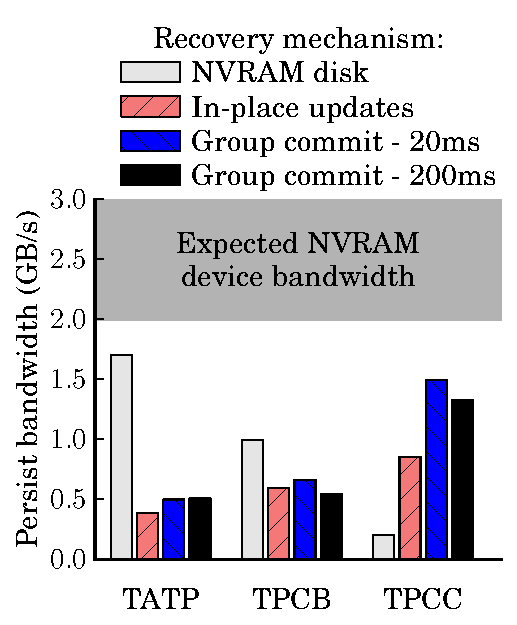
\includegraphics[width=.9\linewidth]{OLTP_eval/Bandwidth.pdf}
  \caption{\textbf{Required NVRAM bandwidth.} Persist/write bandwidth required to achieve 95\% performance relative to no bandwidth constraint.  Bandwidth requirements are far below expected device bandwidth.}
  \label{fig::Bandwidth}
\end{figure}

%Different NVRAM storage architectures impose a variety of limitations on persist bandwidth (e.g., memory bus-attached NVRAM will allow greater throughput than PCIe-attached NVRAM).
%I intend to study the persist bandwidth requirements for each recovery mechanism.
%
%Recovery mechanisms display interesting behaviors with respect to bandwidth.
%\NVDisk persists inefficiently with respect to the total number of bytes updated; even a small page update requires large log entries.
%However, the log persist makes effective use of cache lines (the granularity that data must transfer to the memory device).
%Further, when increased recovery latency is allowable, bandwidth usage may be decreased by deferring page flushing, allowing writes to coalesce in pages.
%The result is that \NVDisk makes reasonable use of bandwidth, and bandwidth constraints are unlikely to limit throughput.
%
%\InPlace displays similar bandwidth usage to \NVDisk.
%All page updates must persist to NVRAM, and these updates tend to use cache lines ineffectively (only a small portion of each cache line changes).
%Also similarly to \NVDisk, \InPlace must maintain ARIES logs (although per-transaction and undo-only), requiring large persists.
%
%\GroupCommit, while persisting the least amount of data, is the most sensitive to persist bandwidth constraints.
%The total quantity of data is reduced by using physical logs -- logs copy data with little associated metadata.
%Additionally, updates in each batch coalesce.
%Only the first write to a given address produces undo, and only the final write to that address persists in-place.
%Other versions of data during the batch do not persist.
%The downside of \GroupCommit is that persists occur in bursts between batches.
%No data persists while the batch executes.
%Between batches however, all logs and heap data persists, placing huge requirements on bandwidth.
%I intend to include a quantitative study of this behavior.
%
%\textbf{Device lifetime.}
%\begin{figure*}
  \centering
  \subfigure[No wear leveling]{\label{fig::WearLeveling::None} 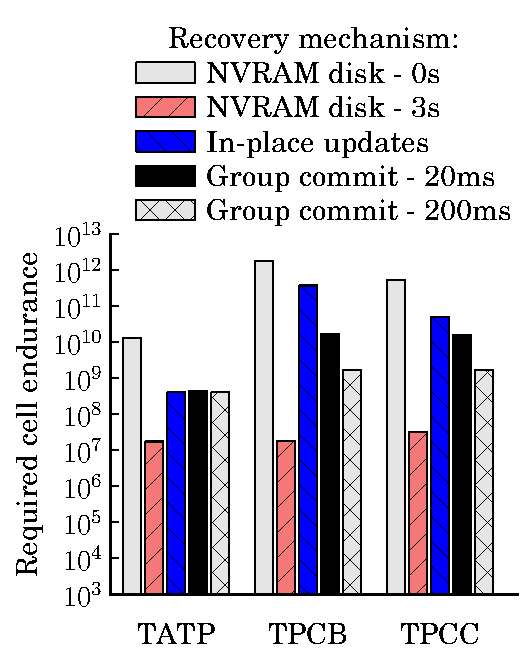
\includegraphics[width=.49\textwidth]{OLTP_eval/WearLeveling_None.pdf}}
  \subfigure[Perfect wear leveling]{\label{fig::WearLeveling::Perfect}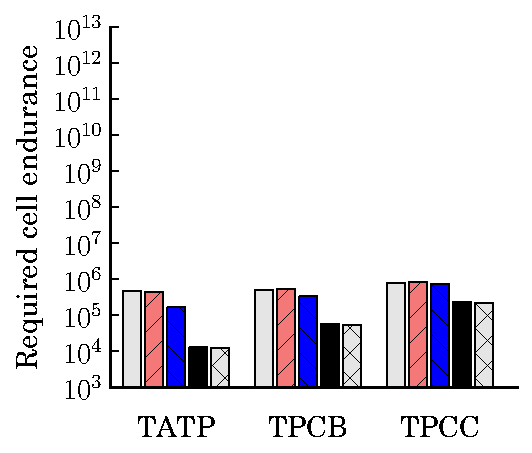
\includegraphics[width=.49\textwidth]{OLTP_eval/WearLeveling_Perfect.pdf}}
  \caption{\textbf{NVRAM cell endurance for 10-year lifetime.}  Without hardware wear leveling the most-written cell limits device lifetime.  \NVDisk requires conservative page flushing (3s recovery latency vs 0s, instantaneous, recovery) and \GroupCommit requires longer batch periods (200ms vs 20ms) to improve device lifetime.  We expect hardware wear leveling to always be required with \InPlace.  With perfect wear leveling (all writes occur evenly throughout cells in the device) and a 32GB storage device all workloads and configurations achieve a 10-year device lifetime for cell endurance of $10^6$ writes and greater.}
  \label{fig::WearLeveling}
\end{figure*}

%NVRAM technologies, much like Flash memory currently, will have limited write endurance; each cell may only be reliably written to a finite number of times.
%Device lifetime is generally determined by the most frequently written addresses.
%Previous work proposes hardware techniques to evenly distribute writes amongst cells by constantly changing the mapping between between memory addresses and the underlying memory cell \cite{QureshiKaridis09}.
%These techniques prolong device lifetime by ensuring that frequently written addresses do not wear out individual cells.
%While the recovery mechanisms presented here each produce varying persist rates with different abilities to naturally distribute persists across addresses, it is unclear if software mechanisms are sufficient to prolong device lifetime.
%I intend to study expected device lifetime for each recovery mechanism, both assuming that persists to an address always persist to the same cell, and assuming hardware that evenly distributes persists across cells.
%
%When wear-leveling hardware is unavailable \NVDisk manages to prolong lifetime the best of the three recovery mechanisms.
%Centralized logs evenly persist to the entire log address space.
%Writes to individual pages may be bounded by limiting the page flush rate, although at the cost of recovery latency.
%\InPlace provides the shortest device lifetime.
%Updates to hot pages and addresses persist each distinct value, quickly wearing out hot cells.
%\GroupCommit limits writes to hot address, but is insufficient to provide lifetime guarantees for expected phase-change write endurance.
%Persists coalesce within each batch, bounding persists to a single write per cell per batch.
%However, batches are sufficiently short that hot addresses still experience a high write-rate, wearing out quickly.
%
%The story changes when hardware spreads persists across NVRAM cells.
%With wear-leveling the primary concern is the total number of persists; all cells experience the same number of persists.
%While \GroupCommit outperforms \NVDisk and \InPlace in this regard, none of the recovery mechanisms pose a device lifetime concern.
%Simply put, an insufficient amount of data persists to worry about device lifetime in the presence of hardware wear-leveling.
%I will include a quantitative evaluation of device lifetime by measuring the rate that persists occur to individual addresses.

\section{Conclusion}
\label{sec:OLTP_eval:Conclusion}
New NVRAM technologies offer an alternative to disk that provides high performance while maintaining durable transaction semantics, yet existing database software is not optimized for such storage devices.
In this chapter, I evaluated recovery management to optimize for NVRAM read and persist characteristics.
I found that even small caches effectively reduce NVRAM read stalls.
I also considered database performance in the presence of persist barrier delays.
Treating NVRAM as a drop-in replacement for disk, \NVDisk retains centralized logging overheads.
\InPlace reduces these overheads, but for large persist barrier latencies suffers from excessive synchronization stalls.
I proposed a new recovery mechanism, \GroupCommit, to minimize these stalls while still removing centralized logging.
While \GroupCommit increases high-percentile transaction latency, latency is controllable and within modern application constraints.
